\documentclass[a4paper, 12pt]{report}

%% Title Definition Packages & Commands %%
\usepackage{titlesec}
\titleformat
{\chapter}
	[display]
	{\bfseries\LARGE}
	{Chapter \thechapter}
	{0pt}
	{
		\rule{\textwidth}{1pt}
		\centering
	}
	[
		\rule{\textwidth}{0.3pt}
	]
\titlespacing{\chapter}{0pt}{10pt}{10pt}
%%%%

\usepackage{enumitem}

\usepackage{fontawesome}

%% Geometry Packages & Commands %%
\usepackage[a4paper]{geometry}
\pdfoutput=1
%%%%

%% ICLR Conference Packages & Commands %%
%% \usepackage{preiclr,times}
\usepackage{iclr2017_conference,times}
\iclrfinalcopy
%%%%

%% Bibliography Package %%
\usepackage[english]{babel}
%%%%

%% Packages from the American Mathematical Society %%
\usepackage{amssymb}
\usepackage{amsfonts}
\usepackage{amsmath}
\usepackage{physics}
%%%%

%% Graphics Packages & Commands %%
\usepackage{graphicx}
\graphicspath{{images/}}
%%%%

%% Font Packages %%
\usepackage[default]{sourcesanspro}
\usepackage[T1]{fontenc}
%%%%

%% Color Package & Command %%
\usepackage{xcolor}
\definecolor{red-secondary-dark}{RGB}{205,32,38}
\definecolor{blue-primary-alt}{RGB}{2,191,231}
\definecolor{red-secondary}{RGB}{227,28,61}
%%%%

%% Reference Packages & Commands %%
\usepackage{url}
\usepackage{hyperref}
\usepackage{cleveref}
\newtheorem{theorem}{Theorem}
\newtheorem{lemma}{Lemma}
\crefname{lemma}{Lemma}{Lemmas}
%%%%

%% Space Packages & Commands %%
\usepackage{setspace}
\newcommand\tab[1][1cm]{\hspace*{#1}}
%%%%

%% Caption Packages & Commands %%
\usepackage[rightcaption]{sidecap}
\usepackage[font={color=red-secondary-dark,small},figurename=Fig.,labelfont={it}]{caption}
\captionsetup[algorithm]{labelsep=colon}
%%%%

%% Box Packages & Commands %%
\usepackage{lmodern}
\usepackage[most]{tcolorbox}
\newtcolorbox[blend into=figures]{blockfigure}[2][]
	{
		colback=white,
		float=!htbp,
		boxsep=1pt,
		left=1pt,
		right=1pt,
		top=1pt,
		bottom=1pt,
		center title,
		%%lifted shadow={1mm}{-2mm}{3mm}{0.1mm}{black!50!white},
		title={#2},
		every float=\centering,
		#1
	}
\newtcolorbox[blend into=figures]{inlinefigure}[2][]
	{
		colback=white,
		boxsep=0.5pt,
		left=1pt,right=1pt,
		top=1pt,
		bottom=1pt,
		center title,
		%%lifted shadow={1mm}{-2mm}{3mm}{0.1mm}{black!50!white},
		title={#2},
		every float=\centering,
		#1
	}
%%%%

%% Code Packages %%
\usepackage{listings}
\usepackage{algorithm}
\usepackage{algorithmicx}
\usepackage{algpseudocode}
%%%%
\usepackage{textcomp}
		
\newtheorem{definition}{Definition}

\newcounter{examplecounter}
\newcommand{\example}[1]{\protect\stepcounter{examplecounter}\textbf{Example~\theexamplecounter:}~#1}


\begin{document}
\begin{titlepage}
	\begin{center}
		\includegraphics[width=0.6\textwidth]{UnivAQ-logo}\\[1cm]
		{\LARGE University of L'Aquila}\\[0.5cm]
		{\large Department of Information Engineering, Computer Science and Mathematics}\\[0.5cm]
		\rule{\linewidth}{0.5mm} \\[0.4cm]
		{\huge \bfseries Hyper Heursitic Cryptography\\
			with\\
			Mixed Adversarial Nets \\[0.4cm] }
		\rule{\linewidth}{0.5mm} \\[0.5cm]
		\noindent
			\begin{tcbraster}[raster columns=2,raster rows=1,
				enhanced,size=small,fit algorithm=hybrid* ]
					\begin{tcolorbox}[
						colback=white,
						sharp corners = northwest,
						title={Author}
						]
							\large
							\emph{Name :} \\[0.2cm]
							\tab Aly \textsc{Shmahell}\\[1cm]
							\emph{Signature :}\\[0.8cm]
							\rule{\linewidth}{0.5mm}
					\end{tcolorbox}
					\begin{tcolorbox}[
						colback=white,
						sharp corners = northwest,
						title = {Supervisor}
						]
							\large
							\emph{Name :} \\[0.2cm]
							\tab Prof.~Giovanni \textsc{De Gasperis}\\[1cm]
							\emph{Signature :}\\[0.8cm]
							\rule{\linewidth}{0.5mm}
					\end{tcolorbox}
			\end{tcbraster}
			\vfill
		\today
	\end{center}
\end{titlepage}
\begin{titlepage}	
	\rule{\linewidth}{0.5mm} \\[0.1cm]
	\begin{minipage}{0.5\textwidth}
		\Large{\textbf{Dissertation License}}
	\end{minipage}
	\begin{minipage}{0.5\textwidth}
		\begin{flushright}
			\includegraphics[angle=-90]{by-nc-sa}
		\end{flushright}
	\end{minipage}
	\\[0.1cm]
	\rule{\linewidth}{0.5mm} \\[0.1cm]
	\noindent
	\begin{center}
		This dissertation (in both source and compiled forms) is licensed under a\\
		\href{http://creativecommons.org/licenses/by-nc-sa/4.0/}{Creative Commons Attribution-NonCommercial-ShareAlike 4.0 International License.}
	\end{center}	
	\rule{\linewidth}{0.5mm} \\[1.5cm]
	\noindent
	\rule{\linewidth}{0.5mm} \\[0.4cm]
	\begin{minipage}{0.5\textwidth}
		\Large{\textbf{Project License}}
	\end{minipage}
	\begin{minipage}{0.5\textwidth}
		\begin{flushright}
			\Huge{\textcopyright}
		\end{flushright}
	\end{minipage}
	\\[0.1cm]
	\rule{\linewidth}{0.5mm} \\[0.1cm]
	\noindent
	\begin{center}
		The code for this dissertation (in both source and compiled forms) is copyrighted under the following terms:
	\end{center}
	\begin{tcbraster}[raster columns=2,raster rows=1,
		enhanced,size=small,fit algorithm=hybrid* ]
		\begin{center}
			\begin{tcolorbox}[colback=white]
				\begin{center}
					Copyright \textcopyright \space 2018, Aly Shmahell.\\
					All rights reserved.
				\end{center}
		\end{tcolorbox}
		\end{center}
	\end{tcbraster}
	\rule{\linewidth}{0.5mm} \\[1.5cm]
	\noindent
	\rule{\linewidth}{0.5mm} \\[0.4cm]
	\begin{minipage}{0.5\textwidth}
		\Large{\textbf{Author's Contact Information}}
	\end{minipage}
	\\[0.1cm]
	\rule{\linewidth}{0.5mm} \\[0.1cm]
	\noindent
	\begin{center}
		\begin{minipage}{0.5\textwidth}
			\faGithub \space:~@AlyShmahell \\
			\faTwitter \space:~ @AlyShmahell \\
			\faLinkedinSquare \space:~ alyshmahell \\
			\faEnvelope \space:~ aly.shmahell@gmail.com
		\end{minipage}
	\end{center}
	\rule{\linewidth}{0.5mm} \\[1.5cm]
	\noindent
	\rule{\linewidth}{0.5mm} \\[0.2cm]
	\begin{minipage}{\textwidth}
		\Large{\textbf{Code Repository \& Dissertation Publication}}
	\end{minipage}
	\rule{\linewidth}{0.5mm} \\[0.1cm]
	\noindent
		\begin{flushleft}
		A Copy of this dissertation can be found on the author's Github account.\\
		A Copy of the code is available for review by academic researchers and industry professionals upon request.
		\end{flushleft}	
	\rule{\linewidth}{0.5mm}
	\noindent
\end{titlepage}
\newpage
\begin{abstract}
\end{abstract}
\newpage
\chapter{Introduction}\label{sec:introduction}
\begin{definition}
	Neural cryptography is an interdisciplinary field in Computer Science, combining both Artificial Intelligence and Cryptography, towards the development of stochastic methods, based on artificial neural networks, for use in encryption and cryptanalysis.
\end{definition}
\section{\textbf{Paper Objectives}}
The objective of this paper is to explore the use of new developments in the field of Neural Networks, mainly Adversarial Neural Networks and Convolutional Neural Networks, as a generative model, to produce a new breed of Crypto-Systems.\\\\
The work being done here is based on a new paper released in 2016 from Google Brain ~\citep{DBLP:journals/corr/AbadiA16}, which promises to bridge the gap between research and application in the area of Neural Cryptography.\\\\
The goal of my research is to provide the following:
\begin{itemize}
	\item An addition to the variety of the underlying mechanics provided in the original paper.
	\item An improvement in performance of the models being built.
	\item An in-depth analysis of how the components work, and the inner details of their mechanics.
	\item A software documentation that provides a blueprint for a more software-engineering oriented neural cryptosystem prototype.
\end{itemize}
With the research paper specter in this area being dominated by authors coming from a mathematical-background angle, my paper aims to provide:
\begin{itemize}
	\item A Computer Science oriented approach to solving cryptography with neural networks and stochastic methods.
\end{itemize}
This paper finally adds the following:
\begin{itemize}
	\item The introduction of a hybrid neural crypto-system.
	\item An exploration into adding hyper heuristics to the field.
\end{itemize}
\newpage
\section{\textbf{Paper Motivation}}
The question of motivation behind an idea can be empirically divided into:
\begin{itemize}[nosep]
	\item How would the author justify the importance of the idea?
	\item How would the author justify the viability of the idea?
\end{itemize}
\subsection{\textbf{Justification for the importance of Neural Cryptography}}
The age of intelligent machines is comprised of multiple intricate components, but individually they function narrowly even for the simplest of tasks. However, the surge of incorporation of these multiple components into one backbone that is neural-nets, has put artificial intelligence on a fast track towards competence in multiple complex areas of problem solving, surpassing traditional methods by multitudes on many occasions.\\\\
It makes sense from an academic perspective that we want neural nets to incorporate an understanding of cryptography, this would propel them closer to achieving general intelligence status, which is a major drive behind research in the field.\\\\
It also makes sense from an economic and existential point that we want neural nets to parallel their success in surpassing traditional methods when it comes to cryptography, because cryptography from a traditional sense is static, it always requires mathematicians and computer scientists to come together to patch it and upgrade it, and it is also always under attack, its mathematical models are always being broken and bent with the advancement in computer-power and the incorporation of new mathematical models into software that can break it.\\
Having neural nets as a dynamic generative model is an opportunity to gain an upper hand on bad actors and put cryptography in a more reactive state to protect our sensitive infrastructure, it would still require research and development, but it would put the neural net as a front line of always devising new ways to mitigate risk and reformulate a cryptographic solution on the fly.
\subsection{\textbf{Justification for the viability of Neural Cryptography}}
This boils down to multiple general factors:
\begin{itemize}[nosep]
	\item \textbf{Neural Nets are viable general function approximaters:} The incorporation of multiple heuristic methodologies into neural nets has made them tackle a rapidly growing heap of complex tasks, cryptography is just another human invention to be caught up with.
	\item \textbf{Neural Nets are becoming faster:} The increasing successful research into using these heuristics not just to compute a complex task, but to do it quickly without loss in accuracy.
	\item \textbf{Neural Nets are becoming available:} The introduction of tools, frameworks and libraries of industrial level to the public which propelled the field of neural networks and made it ever so easy to replicate experiments and improve upon them.
\end{itemize}
Which lead to those paper-related factors:
\begin{itemize}[nosep]
	\item \textbf{Neural Cryptography is viable:} The introduction of Convolutional networks provides a well tested and understood methodology in reducing problems where local spatial relations in the data matter, which is the case for cryptography.
	\item \textbf{Neural Cryptanalysis is viable:} Having a Mixed Convolutional Net with fully connected layers will teach the network to account for global spatial relations as well, which teaches the net to learn and counter cryptanalysis.
	\item \textbf{Neural Cryptography can be fast:} A result of using Convolutions is that the small-sized pattern-finding filter has shared weights (and biases) for all spatial locations which the convolution processes, and this reduces the compute-power required for the whole process compared to other network models.
	\item \textbf{Neural Cryptography is evolved opposite to being patched:} Adversarial computation has been proven to be effective for years in the form of Genetic Algorithms, and adding adversary as a non-supervised generative model provides a better and easier experiment on how to synthesize a new form of cryptography.
\end{itemize}
\newpage
\section{\textbf{Previous Work}}
The work being done so far in Neural Cryptography can be divided to old (pre 2016), and new (post 2016). For the old section, this paper will only list the works and attributions without delving into the details.
\subsection{\textbf{Previous Work - Pre 2016 Era}}
Up until 2010, Neural Nets were a dark alley in the citadel of Artificial Intelligence, mainly due to lack in advancement in back-propagation optimization which made training deep neural nets hard, and the fact that not many people saw the importance of incorporating other areas of Artificial Intelligence into neural nets.\\ From 2010 until 2016, things started changing for the better, but it was 6 years until the developments allowed for new viable research in Neural Cryptography.\\
Therefor the works in the Pre 2016 Era were merely academic curiosities which did not aim to make it into industry, but they provided a key stepping stone for those of us who came into the field at this better-equipped stage.\\\\
The most notable of these works are:
\begin{itemize}[nosep]
	\item The first definition of the Neuro-Cryptography (AI Neural-Cryptography) applied to DES cryptanalysis. ~\citep{s.dourlens.free.fr/AppliedNeuroCryptography}
	\item Permutation parity machines for neural synchronization ~\citep{1751-8121-42-19-195002}
	\item Permutation parity machines for neural cryptography ~\citep{PhysRevE.81.066117}
	\item Successful attack on permutation-parity-machine-based neural cryptography ~\citep{PhysRevE.85.025101}
\end{itemize}
\subsection{\textbf{Previous Work - Post 2016 Era}}
In the period 2010 - 2016, a surge of new ideas came into play in the field of neural nets, new methods of back-propagation optimization proved to be successful for deep-learning, advancement in initialization and activation solved multitudes of problems like the vanishing gradient (or at least mitigated its effect), ...etc, so it was only natural someone would attempt to take another look at Neural Cryptography, and the most notable works are:
\begin{itemize}[nosep]
	\item \textbf{Learning to Protect Communications with Adversarial Neural Cryptography} ~\citep{DBLP:journals/corr/AbadiA16}:\\
	This paper was the corner stone for my work, it was the first to realize the importance of applying Generative Adversarial Nets and succeed in its efforts to build a viable crypto-system.
	\item \textbf{Tensorflow implementation of Adversarial Neural Cryptography} ~\citep{ankeshanand/neural-cryptography-tensorflow}:\\
	Ankesh Anand's Implementation of (Learning to Protect Communications with Adversarial Neural Cryptography) using tensorflow and python is a very informative open-source prototype which I studied before I set on implementing my project.
	\item \textbf{Adversarial Neural Cryptography in Theano} ~\citep{nlml/adversarial-neural-cryptography}:\\
	Liam Schoneveld made an implementation of (Learning to Protect Communications with Adversarial Neural Cryptography) in Theano and python, his results mirror mine to some extent, and his illustrations and break-down of the process is something to consider going over when delving into Neural Cryptography.
\end{itemize}
\newpage
\chapter{Design}\label{sec:design}
This chapter deals with the inner-mechanics of how convolutional neural nets work, which are the building blocks for the adversarial crypto-system presented.\\\\
As a way to illustrate how a ConvNet should be constructed for our purposes, a simplified dummy example is presented and dissected to explain how its components work.\\
\begin{blockfigure}{Xavier Initialization on neuron "n"}
	\begin{center}
		\includegraphics[height = 0.45\textheight]{SimpleNetDiagram}
	\end{center}
\end{blockfigure}\\
This ConvNet has 6 key components which we will go over as the following:
\begin{itemize}[nosep]
	\item Weight Initialization
	\item 1D Convolution
	\item Batches
	\item Activation Functions
	\item Loss Functions
	\item Optimization
\end{itemize}
\newpage
\section{\textbf{Weight Initialization}}
\begin{definition}
	Initialization is the process in which we give some weight values to some neurons in some layer, the overall process, whether done properly or not means the difference between the network converging on a local/global minima, or never converginf at all.
\end{definition}
\subsection{\textbf{Xavier Initialization} ~\citep{DBLP:journals/jmlr/GlorotB10}  }
\begin{lemma}\label{lemma1}
Suppose our net uses the hyperbolic tangent activation function for its neurons:\\
\begin{blockfigure}{example plot of the hyperbolic tangent}
	\[ \includegraphics[width=0.6\textwidth]{tanh} \]
\end{blockfigure}
\begin{itemize}
	\item If the weights start too small, then the signal shrinks as it passes through each layer until it vanishes ~\citep{an-explanation-of-xavier-initialization}, then as it passes deeper in the network with its small values, the layers it enter will become linear, because the output of the hyperbolic tangent is linear with small input values, this means the deeper layers of the net will loose non-linearity.
	\item If the weights start too large, then the signal grows as it passes through each layer until it becomes too large ~\citep{an-explanation-of-xavier-initialization}, then as it passes deeper in the network with its large values, the layers it enter will become saturated, as the output of the hyperbolic tangent is flat with large input values, and this flatness will cause the gradient to become zero, and we will get the vanishing gradient problem.
\end{itemize}
\end{lemma}
\begin{lemma}\label{lemma2}
Having a pre-defined net graph: for each neuron we know the number of inputs and the number of outputs, therefor we can calculate a reasonable weight for the neuron in question based on a normal distribution of a zero mean and a 1/n variance.
\end{lemma}
\begin{lemma}\label{lemma3}
To achieve initialization while avoiding the two obstacles in \cref{lemma1}, we want the variance to remain the same with each passing layer.	
\end{lemma}
\newpage
Suppose we have an input X from a previous layer with n components and a linear neuron with random weights W in the current layer that spits out the same output Y to some neurons in the next layer.
\begin{blockfigure}{Xavier Initialization on neuron "n"}
		\[ \includegraphics[width=0.6\textwidth]{xavier_illustration} \]
\end{blockfigure}
The output of the neuron will have the following equation:
\begin{center}
	\begin{equation}
		Y = W_1X_1 + W_2X_2 + ... + W_n X_n \label{eq:1}
	\end{equation}
\end{center}
To calculate the variance of each component:
\begin{center}
	\begin{equation}
		Var(W_iX_i) = E[X_i]^2 Var(W_i) + E[W_i]^2 Var(X_i) + Var(W_i)Var(X_i) \label{eq:2}
	\end{equation}
\end{center}
Since our inputs and weights come from a normal distribution of zero mean (from \cref{lemma2}):
\begin{center}
	\begin{equation}
		E[X_i]^2 Var(W_i) + E[W_i]^2 Var(X_i) = 0 \implies
		Var(W_iX_i) = Var(W_i)Var(X_i) \label{eq:3}
	\end{equation}
\end{center}
Since the neurons in the same previous layer are all independent, we assume that both $ X_i $ and $ W_i $  are independent and also identically distributed:
\begin{center}
	\begin{equation}
	 Var(Y) = Var(W_1X_1 + W_2X_2 + ... + W_n X_n) = nVar(W_i)Var(X_i) \label{eq:4}
	\end{equation}
\end{center}
In the last equation, we have the variance of the inputs, the variance of the output and the variance of the weights, now we can calculate the variance of the weights from ~\cref{lemma3}:
\begin{center}
	\begin{equation}
	 Var(Y) = Var(X_i) \implies Var(W_i) = \frac{1}{n_{in}} \implies Var(W_i) * n_{in} = 1  \label{eq:5}
	\end{equation}
\end{center}
Now if we go through the same derivation for back-propagation, we get:
\begin{center}
	\begin{equation}
	Var(W_i) = \frac{1}{n_{out}} \implies Var(W_i) * n_{out} = 1 \label{eq:6}
	\end{equation}
\end{center}
To keep the variance of the input gradient \& the output gradient the same, we combine
\eqref{eq:5} \& \eqref{eq:6} and we get:
\begin{center}
	\begin{equation}
	(n_{out} + n_{in}) * Var(W_i) = 2 \implies Var(W_i) = \frac{2}{n_{in} + n_{out}} \label{eq:7}
	\end{equation}
\end{center}
\newpage
\section{\textbf{1D Convolution}}\label{Conv1D}
When looking for examples and literature on Convolution, the vast majority of what is available is on 2D Convolution, and what might be found on 1D convolution is usually done on 1D data with 1D filter~\citep{math-behind-1d-convolution-with-advanced-examples-in-tf}.\\
Therefor, for the purposes of this study, a more complex example will be presented.
\section{\textbf{1D Convolution on Batch 1D Data with (1,2)-D Filters}}
1D Convolution is the process of using a small window to determine local spatial relations over a 1D data sample.\\
At this moment, the best tool available for representing data samples is \textbf{tensors}, and therefor determining local spatial relations amounts to matrix multiplications of the spatial locations inside the data sample tensor by the portion of the filter tensor that fits the location.\\
In order for the convolution to do these multiplications, it \textbf{slides} over one axis of the 1D data sample, the y-axis, the filter also \textbf{slides} itself to fit the location.\\
In order to perform 1D convolution with a 2D filter (having an x-axis and a y-axis), we need to add another axis to both the data and the filter; done by injecting a z-axis into the y-axis, effectively expanding the y-axis over the z-axis. In this case, when the filter \textit{slides} itself, it \textit{slides} over its x-axis.\\
In this format, the window processing is done by multiplying the z-axis of the sample by the y-axis of the filter, over the x-axis of the filter.\\
Every \textit{slide} is done over a fixed length called a stride, and every \textit{slide} represents moving the filter window over to a new spatial location in the sample.\\
If instead of 1 data sample, we have a batch of data samples, we perform convolution on the samples independently. This means the data batch has an extra axis, an x-axis.\\
This way, each time a convolution over a sample is done, the filter resets its \textbf{slided} position to its default, and the convolution \textbf{steps} onto the next sample over the x-axis in the batch.\\
Finally, we end up with a 3D tensor for the batch data, and another 3D tensor for the filter.\\
After the filter is done processing all the samples in the batch, the result tensor will be a 3D tensor with the following dimension lengths:
\begin{itemize}[nosep]
	\item $ result.xAxis.length = batch.xAxis.length $
	\item $ result.yAxis.length = filter.xAxis.length $
	\item $ result.zAxis.length = filter.zAxis.length $
\end{itemize}
Each entry over the x-axis of the result represent a processed sample, and if the z-axis of the result has $ length > 1 $, then each entry over the y-axis represents a feature map of the sample.\\\\
To illustrate how this works, I've chosen a flat representation of the 3D tensors (representing 3D with 2D), mainly because this is how it's done with Numpy, and this is more practical for Computer Scientists.
\begin{blockfigure}{Flat 2D Representation of 3D Tensors - Numpy Style}
		\begin{center}
			\includegraphics[height=0.21\textheight]{numpy-3Dtensor-axis}
		\end{center}
\end{blockfigure}
\newpage
\subsection{\textbf{1D Convolution Algorithm}}
\begin{lemma}\label{lemma4}
	The relation between the dimension lengths of the batch and the filter can be described as the following:
	\begin{itemize}[nosep]
		\item $ filter.xAxis.length >= 1 $
		\item $ filter.yAxis.length = batch.zAxis.length $
		\item $ filter.zAxis.length >= 1 $
	\end{itemize}
\end{lemma}
\begin{lemma}\label{lemma5}
	if $ filter.xAxis.length > batch.yAxis.length $, the filter is offset by an amount of $ filter\_offset =  filter\_x\_axis\_length - batch\_y\_axis\_length $ throughout the convolution process.
\end{lemma}
\begin{algorithm}
	\caption{1D Convolution Pseudo-Code}
	\begin{algorithmic}
		\State $ step = 0 $
		\If{$ filter.xAxis.length >  batch.yAxis.length$}
			\State $ filter.offset =  filter.xAxis.length - batch.yAxis.length $
		\Else
			\State $ filter.offset =  0 $
		\EndIf
		\While {$ step < batch.xAxis.length $}
			\State $ slide = 0 $
				\While {$ slide < batch.yAxis.length $}
					\State $ y = slide $
					\While {$ y <  batch.yAxis.length $}
						\State $ z = 0 $
						\While {$ z < filter.zAxis.length $}
							\begin{align*}
							\tab result[step][y][z]=
							\sum_{x=0}^{x<=filter.xAaxis.length}\biggl\{
							batch[step][x+slide][y] *\\ filter[x-slide+filter.offset][y][z]
							\biggr\} 
							\end{align*}
							\State $ z = z + 1 $
						\EndWhile
						\State $ y = y + 1 $
					\EndWhile
					\State $ slide = slide + 1 $
				\EndWhile
			\State $ step = step + 1 $
		\EndWhile
	\end{algorithmic}
\end{algorithm}
\newpage
\subsection{\textbf{Simple ConvNet Example with 2 Conv Layers}}
This example illustrates how stacked convolutions work, by feeding one Conv Layer output to the next one.\\\\
It also illustrates how 1D convolution works on batch 1D data with 2D (expanded to 3D) filters in each Conv Layer.\\\\
For the sake of simplicity:
\begin{itemize}
	\item We will forsake the use of activation functions between layers.
	\item We will also use weights initialized by hand, chosen arbitrarily.
\end{itemize}
\vspace{0.25\textheight}
\begin{blockfigure}{Simple ConvNet with 2 Conv Layers}
	\begin{center}
		\includegraphics[width=\textwidth]{convLayerExample}
	\end{center}
\end{blockfigure}
\newpage
	{
		
		\color{blue-primary-alt} 
		\rule{2.1cm}{0.4mm}\\[0.2cm]
		\textbf{Conv Layer \#1}\\
		\rule{2.1cm}{0.4mm}
	}\\\\
\tab The example starts off by generating 1D input strings.\\
\begin{tcbraster}[raster columns=3,raster rows=1,
	enhanced,size=small,fit algorithm=hybrid* ]
	\begin{inlinefigure}{First Input String}
		\begin{center}
			\includegraphics[width=0.5\textwidth]{input1}
		\end{center}
	\end{inlinefigure}
	\begin{inlinefigure}{Second Input String}
		\begin{center}
			\includegraphics[width=0.5\textwidth]{input2}
		\end{center}
	\end{inlinefigure}
	\begin{inlinefigure}{Third Input String}
		\begin{center}
			\includegraphics[width=0.5\textwidth]{input3}
		\end{center}
	\end{inlinefigure}
\end{tcbraster}
\begin{tcbraster}[raster columns=2,raster rows=1,
	enhanced,size=small,fit algorithm=hybrid* ]
	\begin{tcolorbox}[frame hidden,colback=white]
		\tab Input strings are then stacked up \tab along the x-axis to form a 2D batch.
	\end{tcolorbox}
	\begin{inlinefigure}{Input Batch}
		\begin{center}
			\includegraphics[width=\textwidth]{input_final}
		\end{center}
	\end{inlinefigure}
\end{tcbraster}

\begin{tcbraster}[raster columns=2,raster rows=1,
	enhanced,size=small,fit algorithm=hybrid* ]
	\begin{tcolorbox}[frame hidden,colback=white]
		\tab Then the batch gets expanded from \tab 2D to 3D along the y-axis (injecting z-\tab axis into y-axis), which means the\\\tab final batch shape becomes (3, 2, 1).
	\end{tcolorbox}
	\begin{inlinefigure}{Reshaped Input Batch}
		\begin{center}
			\includegraphics[width=\textwidth]{input_reshaped}
		\end{center}
	\end{inlinefigure}
\end{tcbraster}
\begin{tcbraster}[raster columns=2,raster rows=1,
	enhanced,size=small,fit algorithm=hybrid* ]
	\begin{tcolorbox}[frame hidden,colback=white]
		\tab Then finally, a filter of shape (2, 1, 2) is \tab provided for the convolution.
	\end{tcolorbox}
	\begin{inlinefigure}{Filter \#1 with arbitrary weights}
		\begin{center}
			\includegraphics[width=0.34\textwidth]{filter1}
		\end{center}
	\end{inlinefigure}
\end{tcbraster}
\newpage
After the input batch tensor and the filter tensor have been generated, the convolution process can begin.\\
\begin{blockfigure}{ Applying the filter to the first sample in the input batch - generating the first value for the first  in the first feature map.}
	\begin{center}
		\includegraphics[width=\textwidth]{firstConvSample_step1}
	\end{center}
\end{blockfigure}
\begin{blockfigure}{ Applying the filter to the first sample in the input batch - generating the second value in the first feature map.}
	\begin{center}
		\includegraphics[width=\textwidth]{firstConvSample_step2}
	\end{center}
\end{blockfigure}
\newpage
\begin{blockfigure}{ Applying the filter to the first sample in the input batch - generating the second feature map.}
	\begin{center}
		\includegraphics[width=\textwidth]{firstConvSample_step3}
	\end{center}
\end{blockfigure}
\begin{blockfigure}{ The entire convolution performed on the batch data.}
		\begin{center}
			\includegraphics[width=\textwidth]{firstConvSample_final}
		\end{center}
\end{blockfigure}
\tab The resulting 3D tensor is of shape (3, 2, 2), and it contains 2 feature maps.
\newpage
	{
		
		\color{blue-primary-alt} 
		\rule{2.1cm}{0.4mm}\\[0.2cm]
		\textbf{Conv Layer \#2}\\
		\rule{2.1cm}{0.4mm}
	}\\\\
To continue with the example, the resulting tensor from \textbf{Conv Layer \#1} will be fed as input to \textbf{Conv Layer \#2}, for this purpose we need a new filter that conforms to the rules of matrix multiplication (taking into account the sliding rule), that is its y-axis has the same length as the z-axis from the tensor we're convolving on.\\\\
And for the sake of making the example closer to real-life usage, we will make the resulting tensor from \textit{Conv Layer \#2} have the same shape as the original input tensor by making the z-axis of the new filter of length 1, which will reduce the number of feature maps from 2 to 1, then by performing dimensionality reduction (squeezing of the z-axis onto the y-axis).\\\\
The shape of the newly constructed filter would be: (var, 2, 1), where $ var >= 1 $, in our example var = 3.
\begin{blockfigure}{The output from the first conv layer becomes input to the second conv layer}
	\begin{center}
		\includegraphics[width=\textwidth]{secondinput_final}
	\end{center}
\end{blockfigure}
\begin{tcbraster}[raster columns=2,raster rows=1,
	enhanced,size=small,fit algorithm=hybrid* ]
	\begin{tcolorbox}[frame hidden,colback=white]
		\tab A filter of shape (3, 2, 1) is provided \tab for the convolution.
	\end{tcolorbox}
	\begin{inlinefigure}{Filter \#2 with arbitrary weights}
		\begin{center}
			\includegraphics[height=0.3\textheight]{filter2}
		\end{center}
	\end{inlinefigure}
\end{tcbraster}
\newpage
After the input batch tensor has been provided the filter tensor has been generated, the convolution process can begin.\\
\begin{blockfigure}{ Extracting the first value from the first sample in the data tensor to the feature map.}
	\begin{center}
		\includegraphics[width=0.9\textwidth]{secondConvSample_step1}
	\end{center}
\end{blockfigure}
\begin{blockfigure}{Extracting the second value from the first sample in the data tensor to the feature map.}
	\begin{center}
		\includegraphics[width=0.9\textwidth]{secondConvSample_step2}
	\end{center}
\end{blockfigure}
\newpage
\begin{blockfigure}{The entire convolution performed on the batch data.}
	\begin{center}
		\includegraphics[width = \textwidth]{secondConvSample_final}
	\end{center}
\end{blockfigure}
\vspace{40pt}
\begin{blockfigure}{squeezing of the z-axis onto the y-axis.}
	\begin{center}
		\includegraphics[width = \textwidth]{squeeze}
	\end{center}
\end{blockfigure}
\vspace{40pt}
\tab The output 3D tensor is of shape (3, 1, 1), and it contains 1 feature maps.\\
\tab The output tensor is similar in shape to the input tensor, as inferred in the example.
\newpage
\section{\textbf{Batches}}
As seen from \cref{Conv1D}, when performing convolutions: we perform each convolution on each data sample separately.\\
Then the question arises: Why is a batch of samples is needed?
The short answer is simply because a batch allows for a good experiment to take place from a statistical point of view.\\\\
When calculating the training error, each net performs mean reduction on each sample error, and a large sample is required for mean reduction, because the standard error of the mean ($ SEM $) can be expressed as:\\
\begin{center}
	\begin{minipage}{0.5\textwidth}
	$ SEM = \dfrac{\sigma}{\sqrt{n}} $\\
	Where:\\
	\tab \space \space $ \sigma: $ the standard deviation of the batch \\
	\tab \space \space $ n: $ the size of the batch 
\end{minipage}
\end{center}
The less the $ SEM $ value is, the more confidence is placed in the accuracy of the mean reduction of training errors.
\section{\textbf{Activation Functions}}
\begin{blockfigure}{ Net Graph Diagram - Alice}
	\begin{center}
		\includegraphics[width = 0.7\textwidth]{tanh_leakyRelu_tanh}
	\end{center}
\end{blockfigure}
\newpage
\begin{blockfigure}{ Net Graph Diagram - Alice}
	\begin{center}
		\includegraphics[width = 0.7\textwidth]{sigmoid_leakyRelu_sigmoid}
	\end{center}
\end{blockfigure}
\begin{blockfigure}{ Net Graph Diagram - Alice}
	\begin{center}
		\includegraphics[width = 0.7\textwidth]{sigmoid_leakyRelu_tanh}
	\end{center}
\end{blockfigure}
\newpage
\chapter{Implementation}\label{sec:implementation}
\newpage
\begin{blockfigure}{ Net Graph Diagram - Alice}
	\begin{center}
		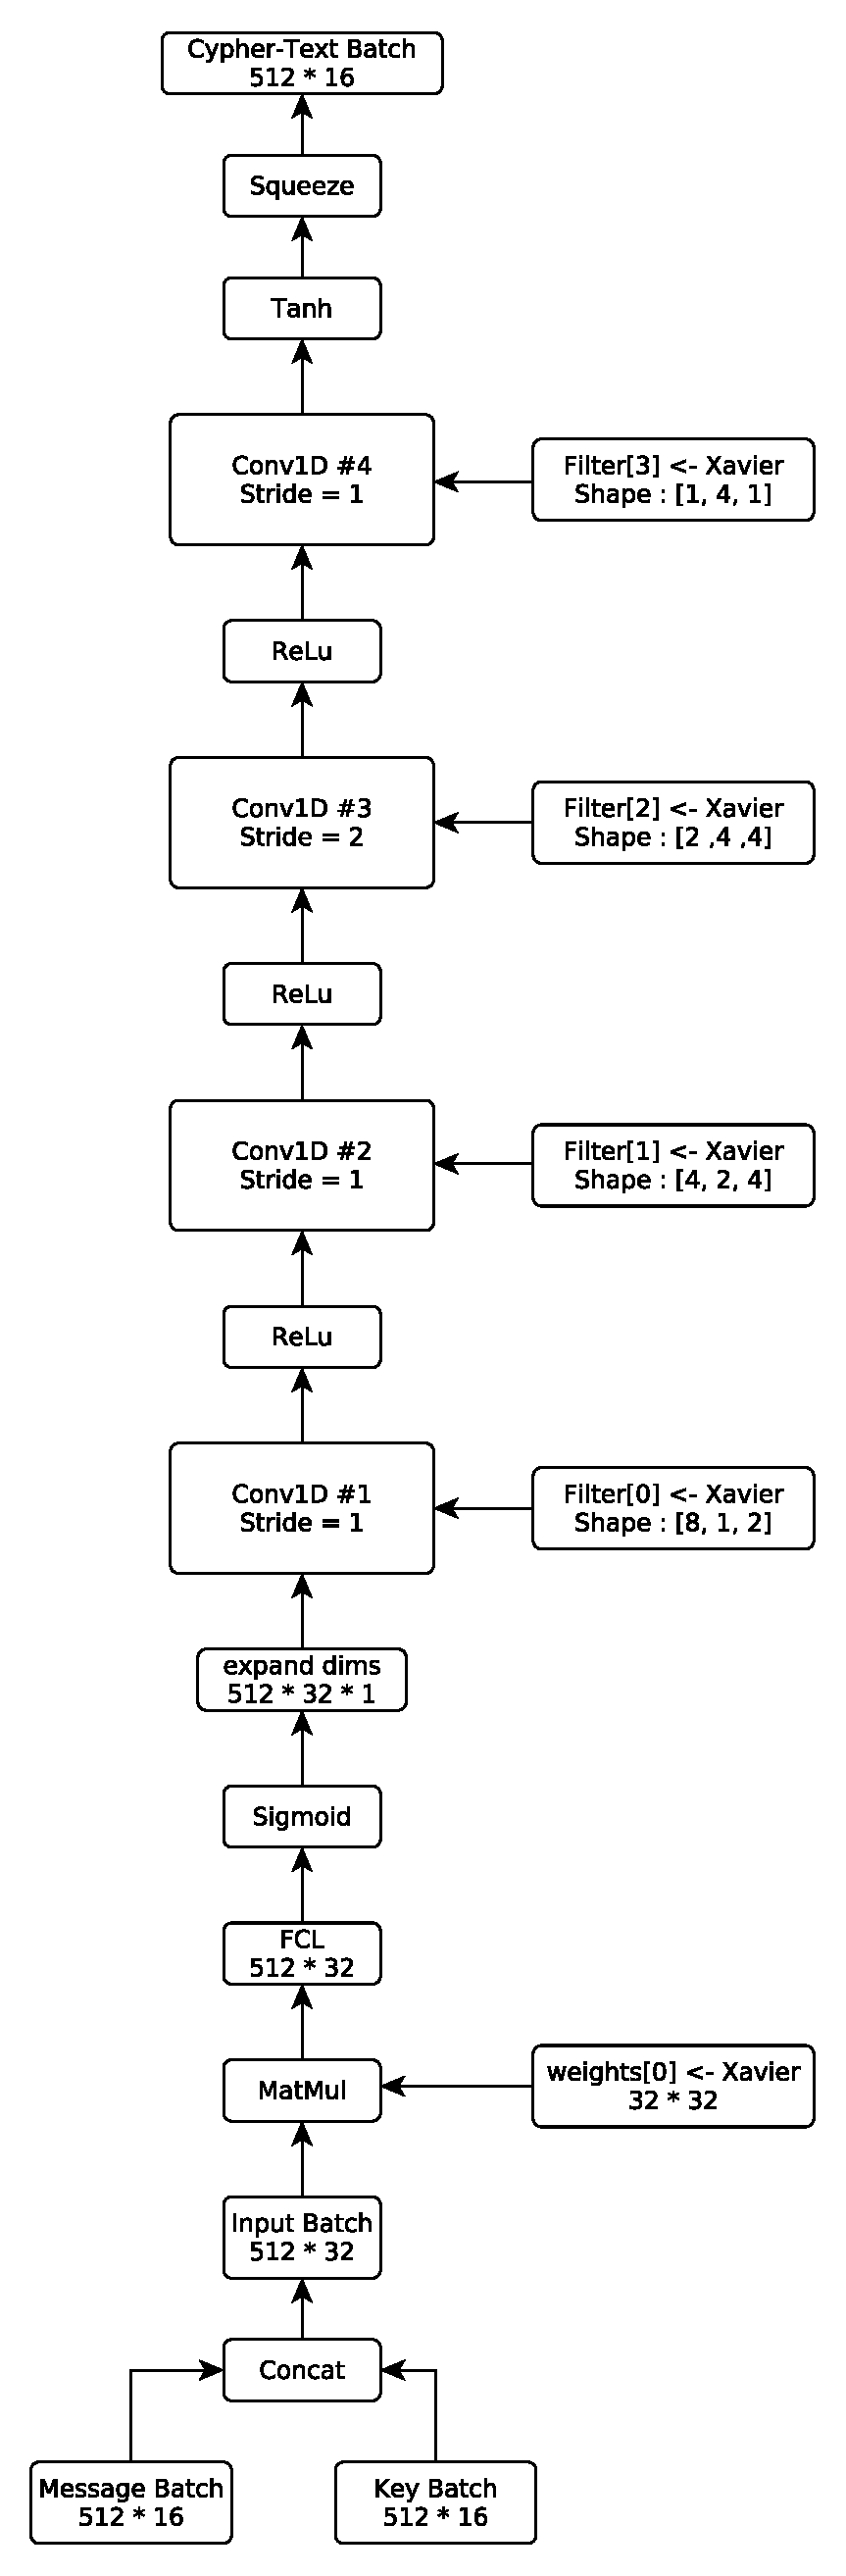
\includegraphics[height=0.93\textheight]{Alice-Diagram}
	\end{center}
\end{blockfigure}
\newpage
\begin{blockfigure}{ Net Graph Diagram - Bob}
	\begin{center}
		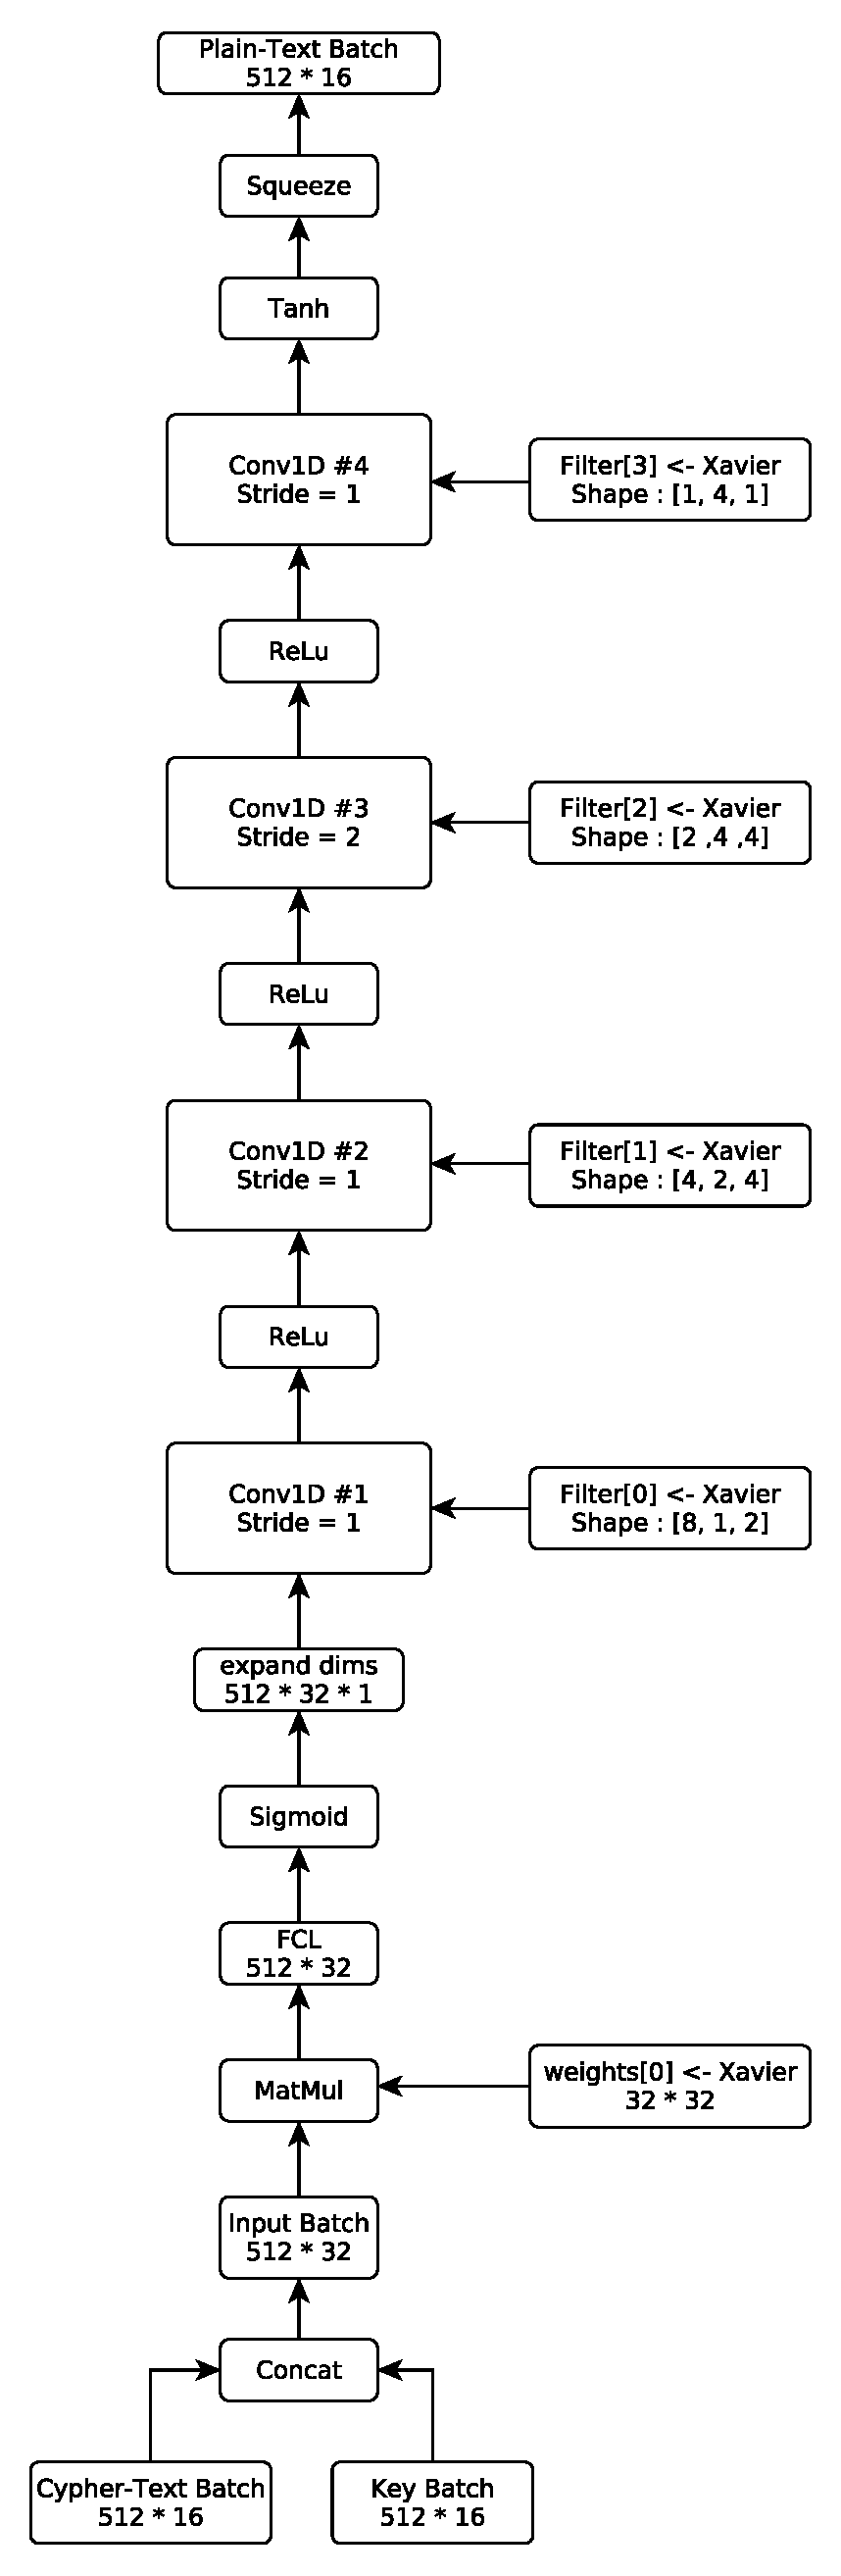
\includegraphics[height=0.93\textheight]{Bob-Diagram}
	\end{center}
\end{blockfigure}
\newpage
\begin{blockfigure}{ Net Graph Diagram - Eve/Alan}
		\begin{center}
			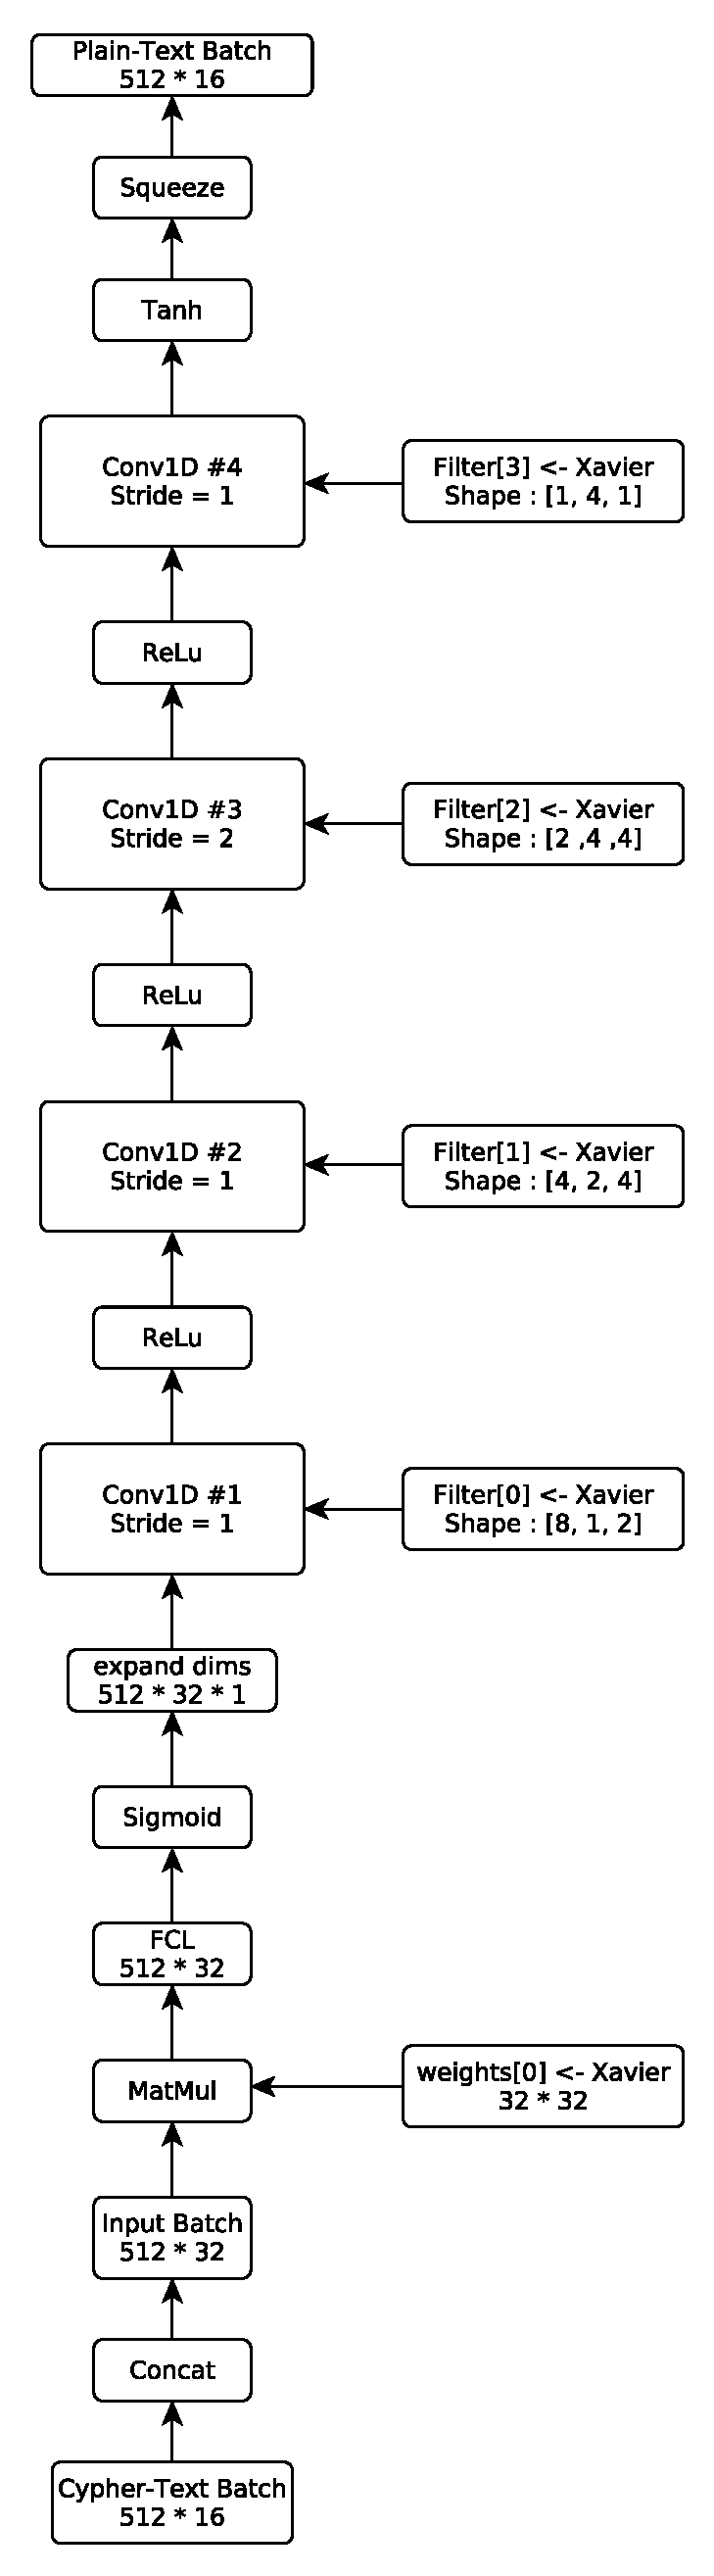
\includegraphics[height=0.93\textheight]{Eve-Diagram}
		\end{center}
\end{blockfigure}
\newpage
\begin{blockfigure}{ Symmetric Scheme}
	\begin{center}
		\includegraphics[width = \textwidth]{symmetricScheme}
	\end{center}
\end{blockfigure}
\newpage
\begin{blockfigure}{ Asymmetric Scheme}
	\begin{center}
		\includegraphics[width = \textwidth, height = 0.98\textheight]{asymmetricScheme}
	\end{center}
\end{blockfigure}
\newpage
\begin{blockfigure}{ Hybrid Scheme}
	\begin{center}
		\includegraphics[width = \textwidth]{hybridScheme}
	\end{center}
\end{blockfigure}
\newpage
\chapter{Conclusion}\label{sec:conclusion}
\newpage
\appendix
\chapter*{Appendix}

\newpage
\medskip
\bibliographystyle{unsrt}
\bibliography{neurencoder}
\end{document}